% The hierarchical model behind the joint posterior: the parameters set the distribution of the
% latent field, and both set the data. Shaded node: observed; white nodes: inferred.
% Compile: pdflatex hierarchical_model.tex && pdftocairo -svg hierarchical_model.pdf hierarchical_model.svg
\documentclass[tikz,border=4pt]{standalone}
\usepackage{tikz}
\usepackage{amsmath}
\usepackage[T1]{fontenc}
\usetikzlibrary{arrows.meta}

\definecolor{ink}{HTML}{2E2E2E}
\definecolor{flow}{HTML}{3B6FB6}
\definecolor{obs}{HTML}{C9D6E6}

\begin{document}
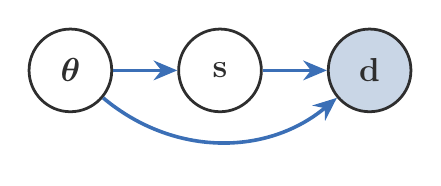
\begin{tikzpicture}[
  var/.style={circle,draw=ink,line width=1pt,minimum size=1.05cm,fill=white,text=ink,font=\large},
  arr/.style={-{Stealth[length=3mm,width=2.5mm]},line width=1.3pt,draw=flow},
]
  \node[var] (th) at (0,0) {$\boldsymbol\theta$};
  \node[var] (s)  at (1.9,0) {$\mathbf{s}$};
  \node[var,fill=obs] (d) at (3.8,0) {$\mathbf{d}$};
  \draw[arr] (th) -- (s);
  \draw[arr] (s) -- (d);
  \draw[arr] (th) to[out=-40,in=-140] (d);
\end{tikzpicture}
\end{document}
